%  template.tex for Biometrics papers
%
%  This file provides a template for Biometrics authors.  Use this
%  template as the starting point for creating your manuscript document.
%  See the file biomsample.tex for an example of a full-blown manuscript.

%  ALWAYS USE THE referee OPTION WITH PAPERS SUBMITTED TO BIOMETRICS!!!
%  You can see what your paper would look like typeset by removing
%  the referee option.  Because the typeset version will be in two
%  columns, however, some of your equations may be too long. DO NOT
%  use the \longequation option discussed in the user guide!!!  This option
%  is reserved ONLY for equations that are impossible to split across 
%  multiple lines; e.g., a very wide matrix.  Instead, type your equations 
%  so that they stay in one column and are split across several lines, 
%  as are almost all equations in the journal.  Use a recent version of the
%  journal as a guide. 
%  
\documentclass[useAMS,usenatbib]{biom}
\usepackage{graphicx}
\usepackage{amsmath}
%\usepackage{amssymb}
%documentclass[useAMS]{biom}
%
%  If your system does not have the AMS fonts version 2.0 installed, then
%  remove the useAMS option.
%
%  useAMS allows you to obtain upright Greek characters.
%  e.g. \umu, \upi etc.  See the section on "Upright Greek characters" in
%  this guide for further information.
%
%  If you are using AMS 2.0 fonts, bold math letters/symbols are available
%  at a larger range of sizes for NFSS release 1 and 2 (using \boldmath or
%  preferably \bmath).
% 
%  Other options are described in the user guide. Here are a few:
% 
%  -  If you use Patrick Daly's natbib  to cross-reference your 
%     bibliography entries, use the usenatbib option
%
%  -  If you use \includegraphics (graphicx package) for importing graphics
%     into your figures, use the usegraphicx option
% 
%  If you wish to typeset the paper in Times font (if you do not have the
%  PostScript Type 1 Computer Modern fonts you will need to do this to get
%  smoother fonts in a PDF file) then uncomment the next line
%  \usepackage{Times}

%%%%% PLACE YOUR OWN MACROS HERE %%%%%

\def\bSig\bmath{\Sigma}
\newcommand{\VS}{V\&S}
\newcommand{\tr}{\mbox{tr}}

\begin{document}

%  This will produce the submission and review information that appears
%  right after the reference section.  Of course, it will be unknown when
%  you submit your paper, so you can either leave this out or put in 
%  sample dates (these will have no effect on the fate of your paper in the
%  review process!)


%\date{{\it Received October} 2007. {\it Revised February} 2008.  {\it
%Accepted March} 2008.}

%  These options will count the number of pages and provide volume
%  and date information in the upper left hand corner of the top of the 
%  first page as in published papers.  The \pagerange command will only
%  work if you place the command \label{firstpage} near the beginning
%  of the document and \label{lastpage} at the end of the document, as we
%  have done in this template.

%  Again, putting a volume number and date is for your own amusement and
%  has no bearing on what actually happens to your paper!  


\label{firstpage}

\section*{Normal Distribution $\mathcal{N}_p(\tilde{\mu},q)$}
%The specification of the mean and variance of a normal distribution completely specifies the modal value and a tail-probability constraint, and is therefore sufficient for defining enthusiastic and skeptical priors.

%\begin{mydef}\label{def:normal}
Define $\theta\sim\mathcal{N}_p(\tilde{\mu},q)$ as the normal distribution $\mathcal{N}(\mu,\sigma)$ that satisfies $\rmn{mode}(\theta)=\tilde{\mu}$ and $P(\theta\leq q)=p$.
%\end{mydef}
%
The values for the mean and standard deviation are solved analytically as $\mu=\tilde{\mu}$ and $\sigma=\frac{q-\mu}{\Phi^{-1}(p)}$, where $\Phi$ denotes the cumulative distribution function for a standard normal distribution, and $\Phi^{-1}$ denotes its quantile function. The distribution $\mathcal{N}_p(\tilde{\mu},q)$ is well-defined for values $(\mu,q,p)$ that satisfy $\frac{q-\mu}{p-0.5}>0$.


 Since the normal distribution is completely specified by $(\mu, \sigma)$, quantities such as $P(\theta\leq\tilde{q})$ are also specified for any $\tilde{q}$. In particular, if $\theta\sim\mathcal{N}_p(\tilde{\mu},q)$ then $P(\theta\leq\frac{q+\mu}{2})=\Phi(\frac{\Phi^{-1}(p)}{2})$. Furthermore, $P(\theta\in(\mu,\frac{q+\mu}{2}))=|p-\Phi(\frac{\Phi^{-1}(p)}{2})|$. 

\section*{Generalized Normal Distribution $\mathcal{GN}(\mu,\alpha,\beta)$}
The pdf and cdf for a generalized normal distribution $\mathcal{GN}(\mu,\alpha,\beta)$ are

\begin{align*}
f(\theta)&=\frac{\beta}{2\alpha\Gamma(1/\beta)}\exp\{-(\frac{|\theta-\mu|}{\alpha})^\beta\}\\
F(\theta)&=\frac{1}{2}+\text{sign}(x-\mu)\frac{\gamma(\frac{1}{p},\frac{|x-\mu|^p}{2\alpha^p})}{2\Gamma(\frac{1}{p})}
\end{align*} where $\mu$ is a location parameter, $\alpha>0$ is a scale parameter, and $\beta>0$ is a shape parameter, $\Gamma(x)=\int_0^\infty t^{x-1}e^{-t}dt$, and $\gamma(x,a)=\int_0^a t^{x-1}e^{-t}dt$ \citep{Nadarajah2005}.

\section*{Generalized Normal Distribution $\mathcal{GN}_p(\tilde{\mu},q,k)$}
%\begin{mydef}\label{def:gennormal}
Define $\theta\sim\mathcal{GN}_p(\tilde{\mu},q,k)$ as the generalized normal distribution $\mathcal{GN}(\mu,\alpha,\beta)$ that satisfies mode$(\theta)=\tilde{\mu}$, $P(\theta\leq q)=p$, and $P(\theta\in(q,\frac{q+\mu}{2}))=k\cdot|p-\Phi(\frac{\Phi^{-1}(p)}{2})|$.
%\end{mydef}
%
The mode is equal to $\mu=\tilde{\mu}$, and $\alpha$ and $\beta$ are determined to minimize the function 
\begin{align*}
(F_{\mu,\alpha,\beta}(q)-p)^2+(F_{\mu,\alpha,\beta}(\frac{q+\mu}{2})-k\cdot|p-\Phi(\frac{\Phi^{-1}(p)}{2})|)^2
\end{align*} with box-constrained optimization \citep{Byrd1995}. 

\section*{Problem}
Prove existence and uniqueness of a $\mathcal{GN}_p(\tilde{\mu},q,k)$ distribution among well-defined choices of $(p,\tilde{\mu},q,k)$.


%The flexibility to modify $\gamma$ can change the distribution to be flatter or more concentrated around the modal value. Choosing $\gamma=1$ corresponds to the normal distribution which is viewed as a default choice. If $\gamma>1$ then the probability that $\theta\in(q,\frac{q+\mu}{2})$ increases and the concentration of $\theta$ around the modal value $\mu$ accordingly decreases, resulting in a flatter distribution around the modal value. If $\gamma<1$ then the probability that $\theta\in(q,\frac{q+\mu}{2})$ decreases and the concentration of $\theta$ around the modal value $\mu$ accordingly increases, resulting in a more concentrated distribution around the modal value. Note that the tail probability $P(\theta\leq q)=p$ is maintained regardless of the choice of $\gamma$. 
%
%Flattening or concentrating the distribution around the modal value is useful for specifying monitoring priors that reflect varying opinions about the dispersion of $\theta$. An example of parameterizing an enthusiastic prior with a $\mathcal{GN}_p(\tilde{\mu},q,\gamma)$ distribution is demonstrated in Figure \ref{fig:figure1}. Choosing a concentrated distribution is appropriate when prior belief reflects a higher degree of certainty that $\theta$ is in a narrow range around $\theta_1$, while maintaining residual uncertainty that $\theta<\theta_0$. This decreases the variance of the distribution, and can be seen to reflect a conservative opinion about the values of $\theta$. Choosing a flattened distribution is appropriate when $\theta$ is more likely to be in a wide range of values around $\theta_1$, while maintaining the same residual uncertainty that $\theta<\theta_0$. This increases the variance of the distribution, and can be seen to reflect a liberal opinion about the values of $\theta$. The specification of $\gamma=0.75$ will be used henceforth as a pre-determined value for creating a concentrated distribution, and $\gamma=1.5$ will be used for creating a flattened distribution. These values of $\gamma$ are chosen based on the intuitive graphical properties of the distribution (e.g. noticeably peaked around $\theta_1$, relatively flat around $\theta_1$). Alternatively, the choice of $\gamma$ could be specified to identify an additional probability constraint exactly (e.g. $P(\theta\in(\theta_0,\frac{\theta_0+\theta_1}{2}))=0.1$). The impact of flattening or concentrating the distribution of a monitoring prior on the operating characteristics of a trial is shown in Section \ref{sec:examples}.

%\subsubsection{Truncated Generalized Normal Distribution $\mathcal{GN}_{p,\Theta}(\tilde{\mu},q,\gamma)$}
%The density for a generalized normal distribution truncated to the interval domain $\Theta=(\theta_{min},\theta_{max})$, denoted by $\mathcal{GN}_\Theta(\mu,\alpha,\beta)$, is $f(\theta)=c\cdot\exp\left\{-\frac{|\theta-\mu|}{\alpha}^{\beta}\right\}{I(\theta\in \Theta)}$ where $c=\frac{\beta}{2\alpha \Gamma(1/\beta)}({F_{\mu,\alpha,\beta}(\theta_{max})-F_{\mu,\alpha,\beta}(\theta_{min})})^{-1}$. 
%
%%\begin{mydef}\label{def:gennormaltruncated}
%Define $\theta\sim\mathcal{GN}_{p,\Theta}(\tilde{\mu},q,\gamma)$ as the truncated generalized normal distribution $\mathcal{GN}_\Theta(\mu,\alpha,\beta)$ that satisfies mode$(\theta)=\tilde{\mu}$, $P(\theta\leq q)=p$, and $P(\theta\in(q,\frac{q+\mu}{2}))=\gamma|p-\Phi(\frac{\Phi^{-1}(p)}{2})|$.
%%\end{mydef}
%%
%For example, consider creating skeptical and enthusiastic priors for a response probability on domain $[0,1]$, as $
%\pi_S(\theta)=\mathcal{GN}_{p=1-\epsilon,\Theta=[0,1]}(\tilde{\mu}=\theta_0,q=\theta_1,\gamma=1)$ and $
%\pi_E(\theta)=\mathcal{GN}_{p=\epsilon,\Theta=[0,1]}(\tilde{\mu}=\theta_1,q=\theta_0,\gamma=1)$ respectively.
\begin{figure}
\begin{center}
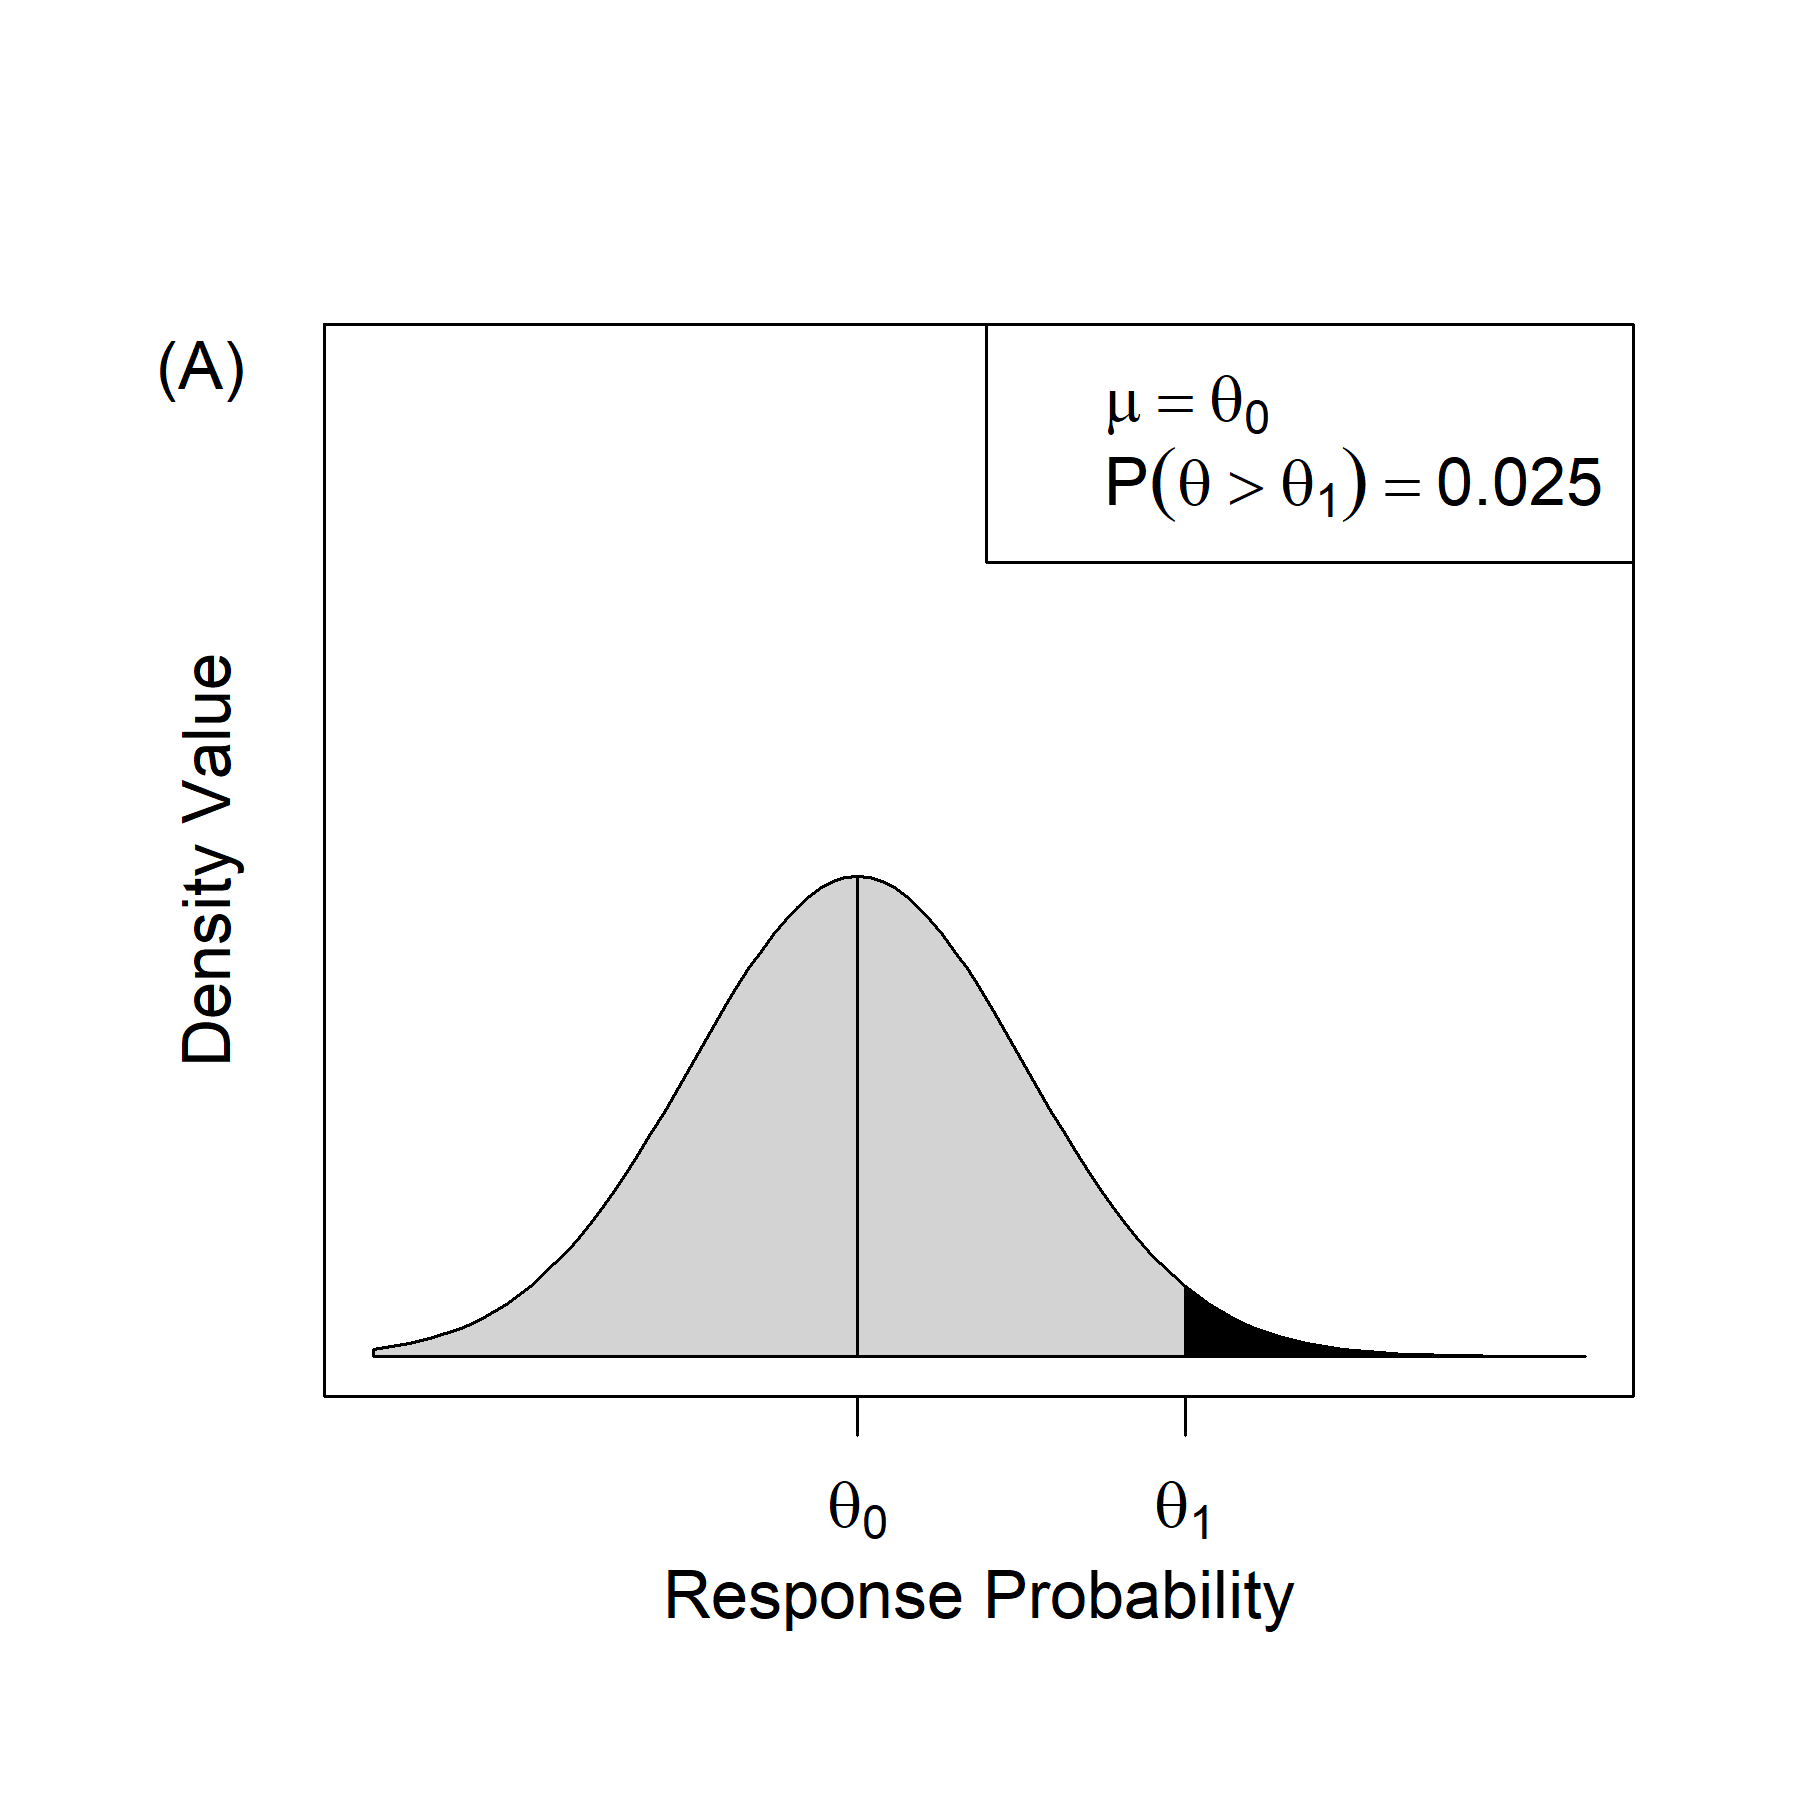
\includegraphics[width=2.9in]{../00-paper/FIGURES/figure1a.png}
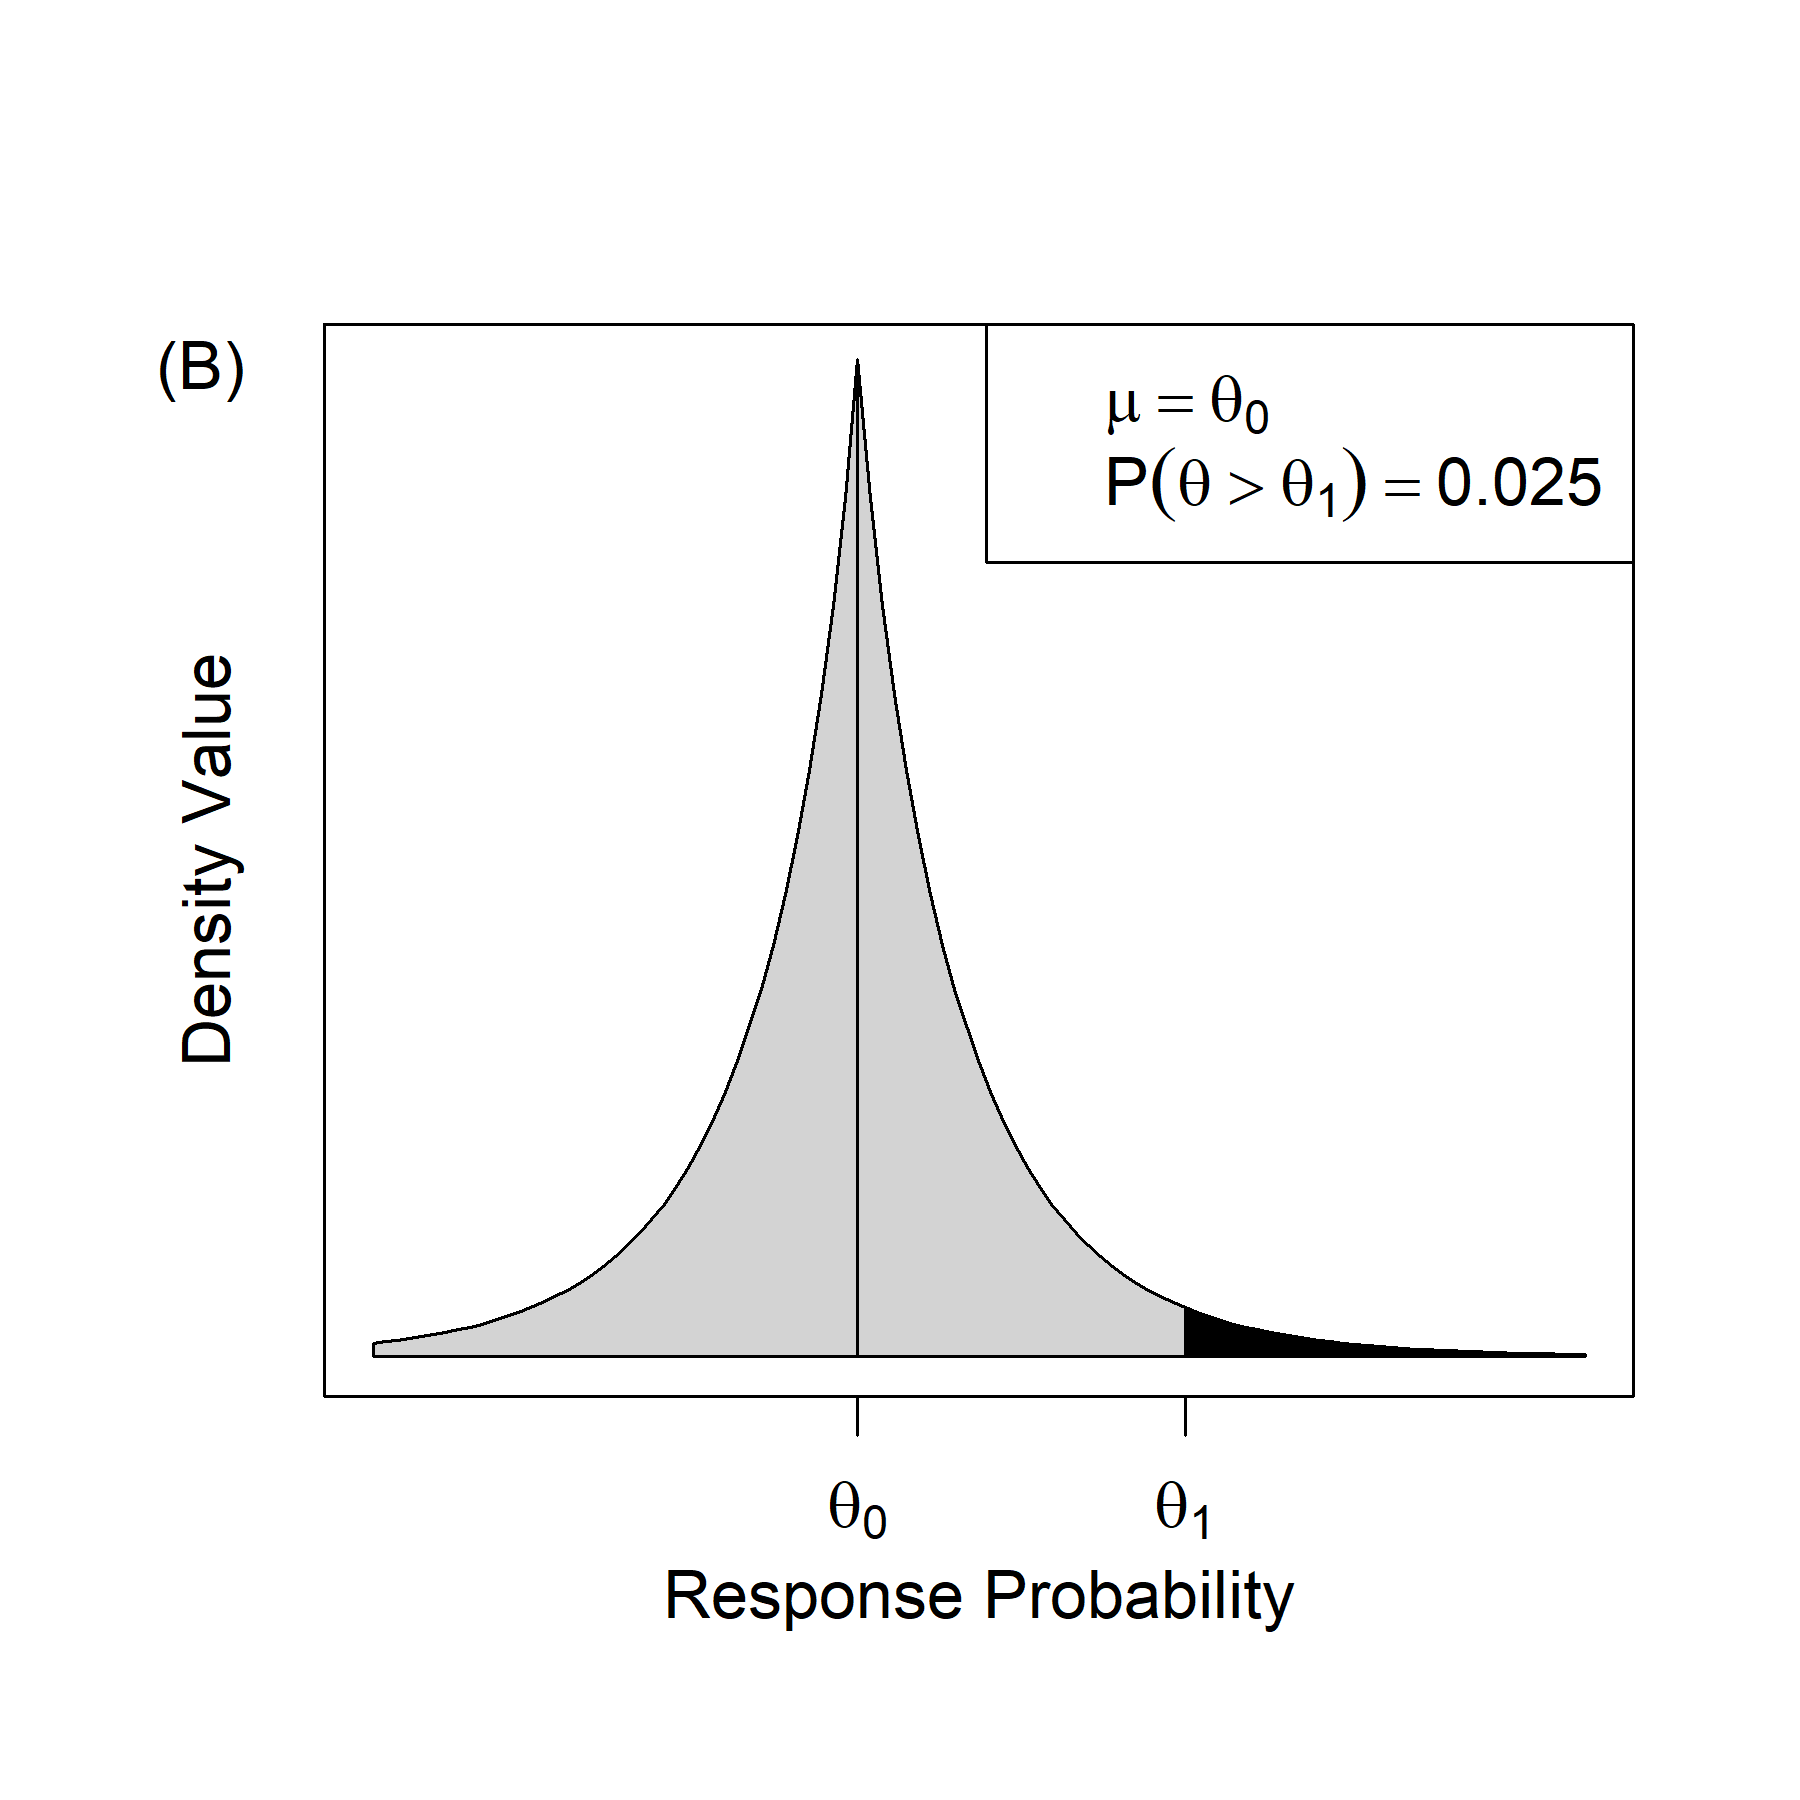
\includegraphics[width=2.9in]{../00-paper/FIGURES/figure1b.png}
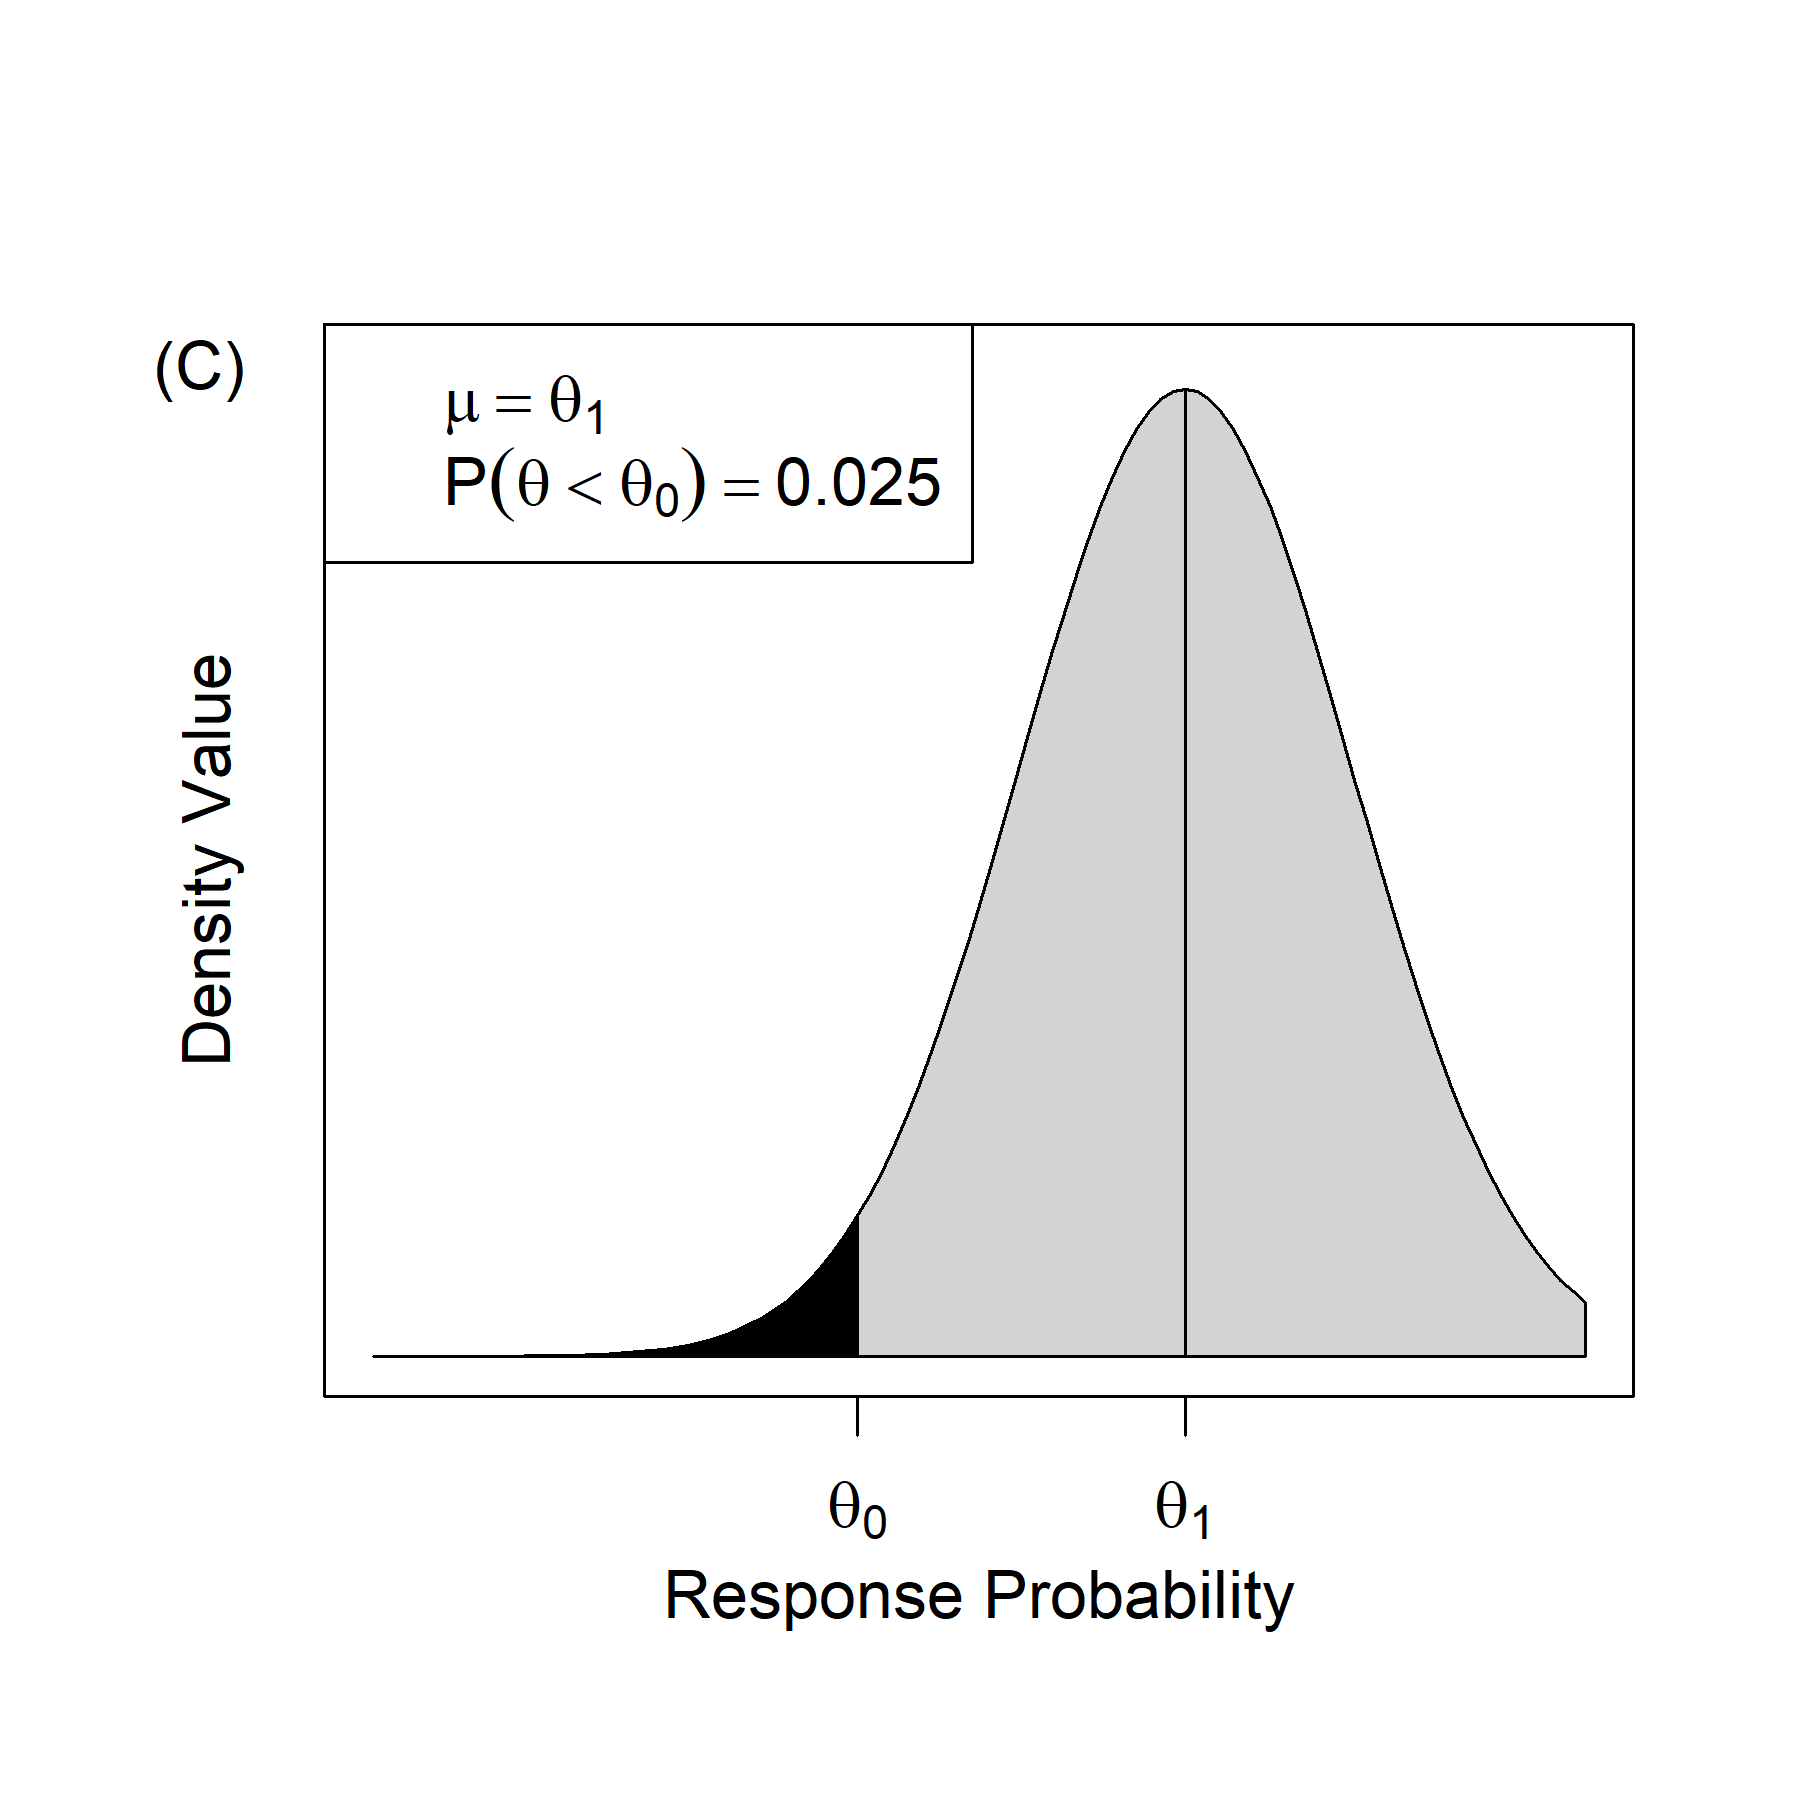
\includegraphics[width=2.9in]{../00-paper/FIGURES/figure1c.png}
\caption{A, $\mathcal{GN}_{p=0.025}(\tilde{\mu}=\theta_1,q=\theta_0,\gamma=1)$. B, $\mathcal{GN}_{p=0.025}(\tilde{\mu}=\theta_1,q=\theta_0,\gamma=0.75)$, C, $\mathcal{GN}_{p=0.025}(\tilde{\mu}=\theta_1,q=\theta_0,\gamma=1.5)$}
\label{fig:figure1}
\end{center}
\end{figure}
%The normal and generalized normal family of distributions can be truncated to a restricted domain that reflects the research quantity of interest (e.g. a response probability on [0,1]).
%\subsubsection{Application to higher dimensions}
%Suppose the trial from Section \ref{sec:preliminaries} has added a control arm, and let $\eta_0$ and $\eta_1$ be the response proportions for a control and treatment group respectively. Suppose that the risk difference $\theta=\eta_1-\eta_0$ is the parameter of interest, and let $\eta_0$ be a nuisance parameter. Let $\delta_0$ denote a null risk difference and $\delta_1$ denote a highly efficacious risk difference.

%The generalized normal distribution can be used to parameterize skeptical and enthusiastic priors for trials with multiple unknown quantities of interest. Let $\theta$ be the parameter of interest and $\eta$ be the nuisance parameters. Consider the following representation of the joint prior for $\theta$ and $\eta$: $\pi(\theta,\eta)=\pi(\theta)\times\pi(\eta|\theta)$. For example, suppose that $\theta$ is the risk difference between response probabilities of the treatment group and the placebo group $\eta$. The distribution for the risk difference is $
%\pi(\theta)\sim\mathcal{GN}_{p,\Theta=[-1,1]}()$. The domain of $\eta$ is $[0,1-\theta)$ if $\theta\geq 0$ and $(-\theta,1)$ if $\theta < 0$. Define the prior for $\eta$ to be $\pi(\eta|\theta)\sim \mathcal{GN}_{p,H=[\rmn{max}(-\theta,0),\rmn{min}(1,1+\theta)]}()$. This prior specification is demonstrated in Figure \ref{fig:figure5}, and Section \ref{sec:example2model} uses this representation of the joint prior.



%\begin{figure}\begin{center}
%%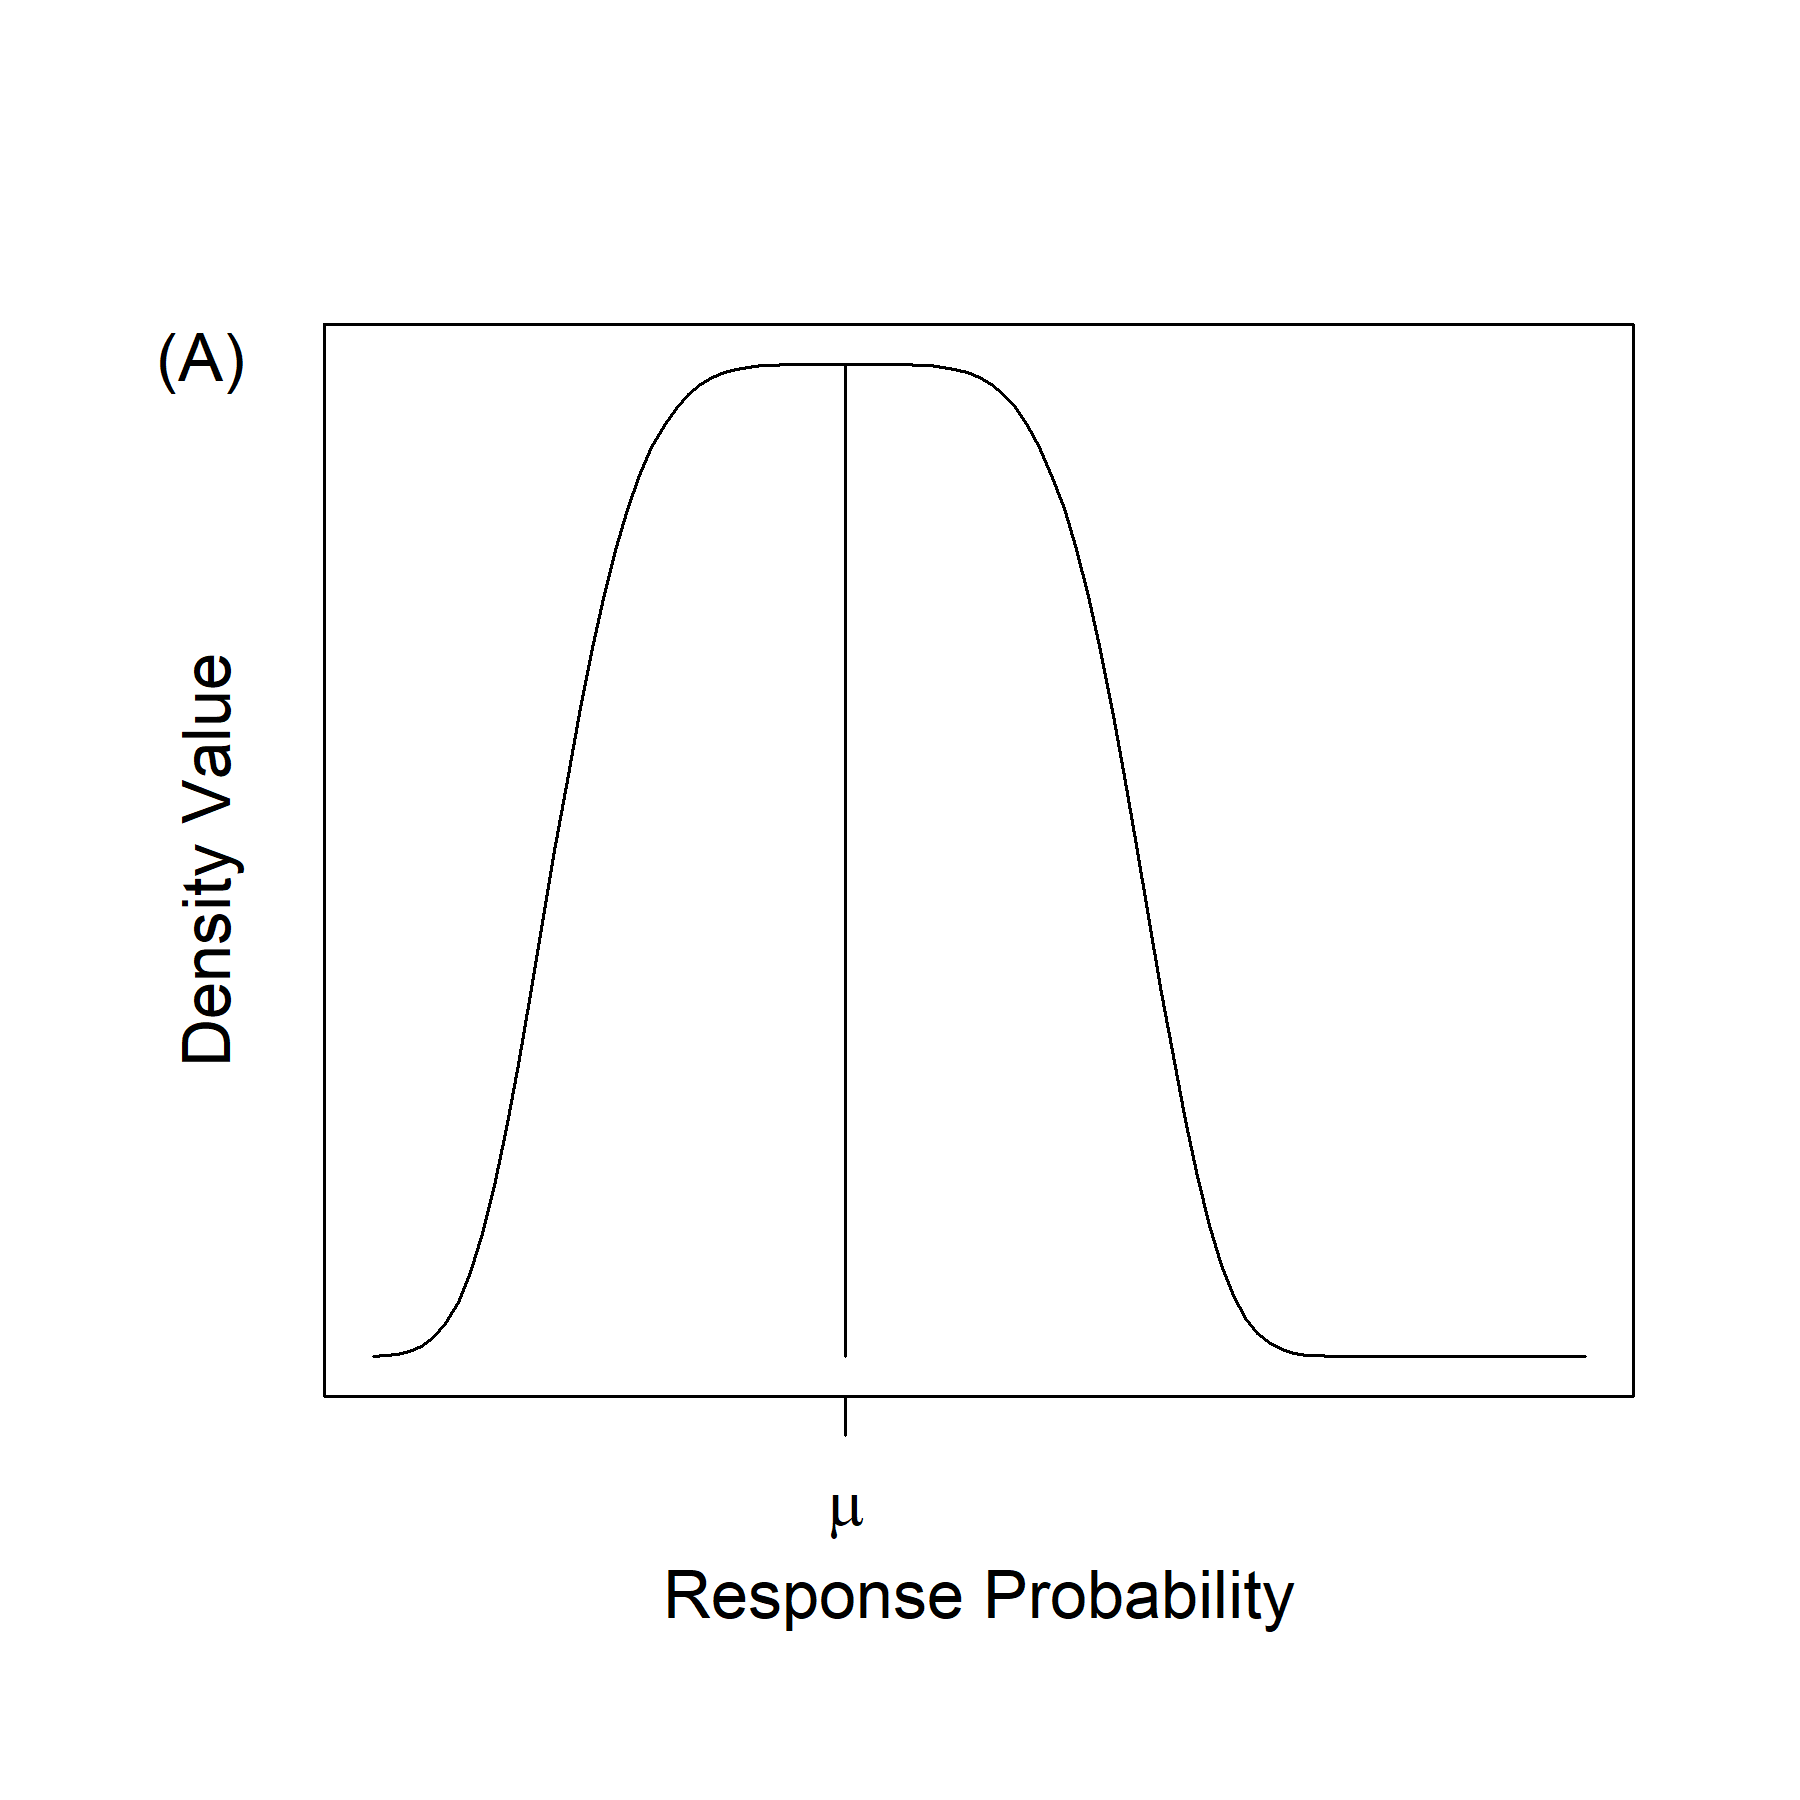
\includegraphics[width=3in]{../00-paper/FIGURES/figure5c.png}
%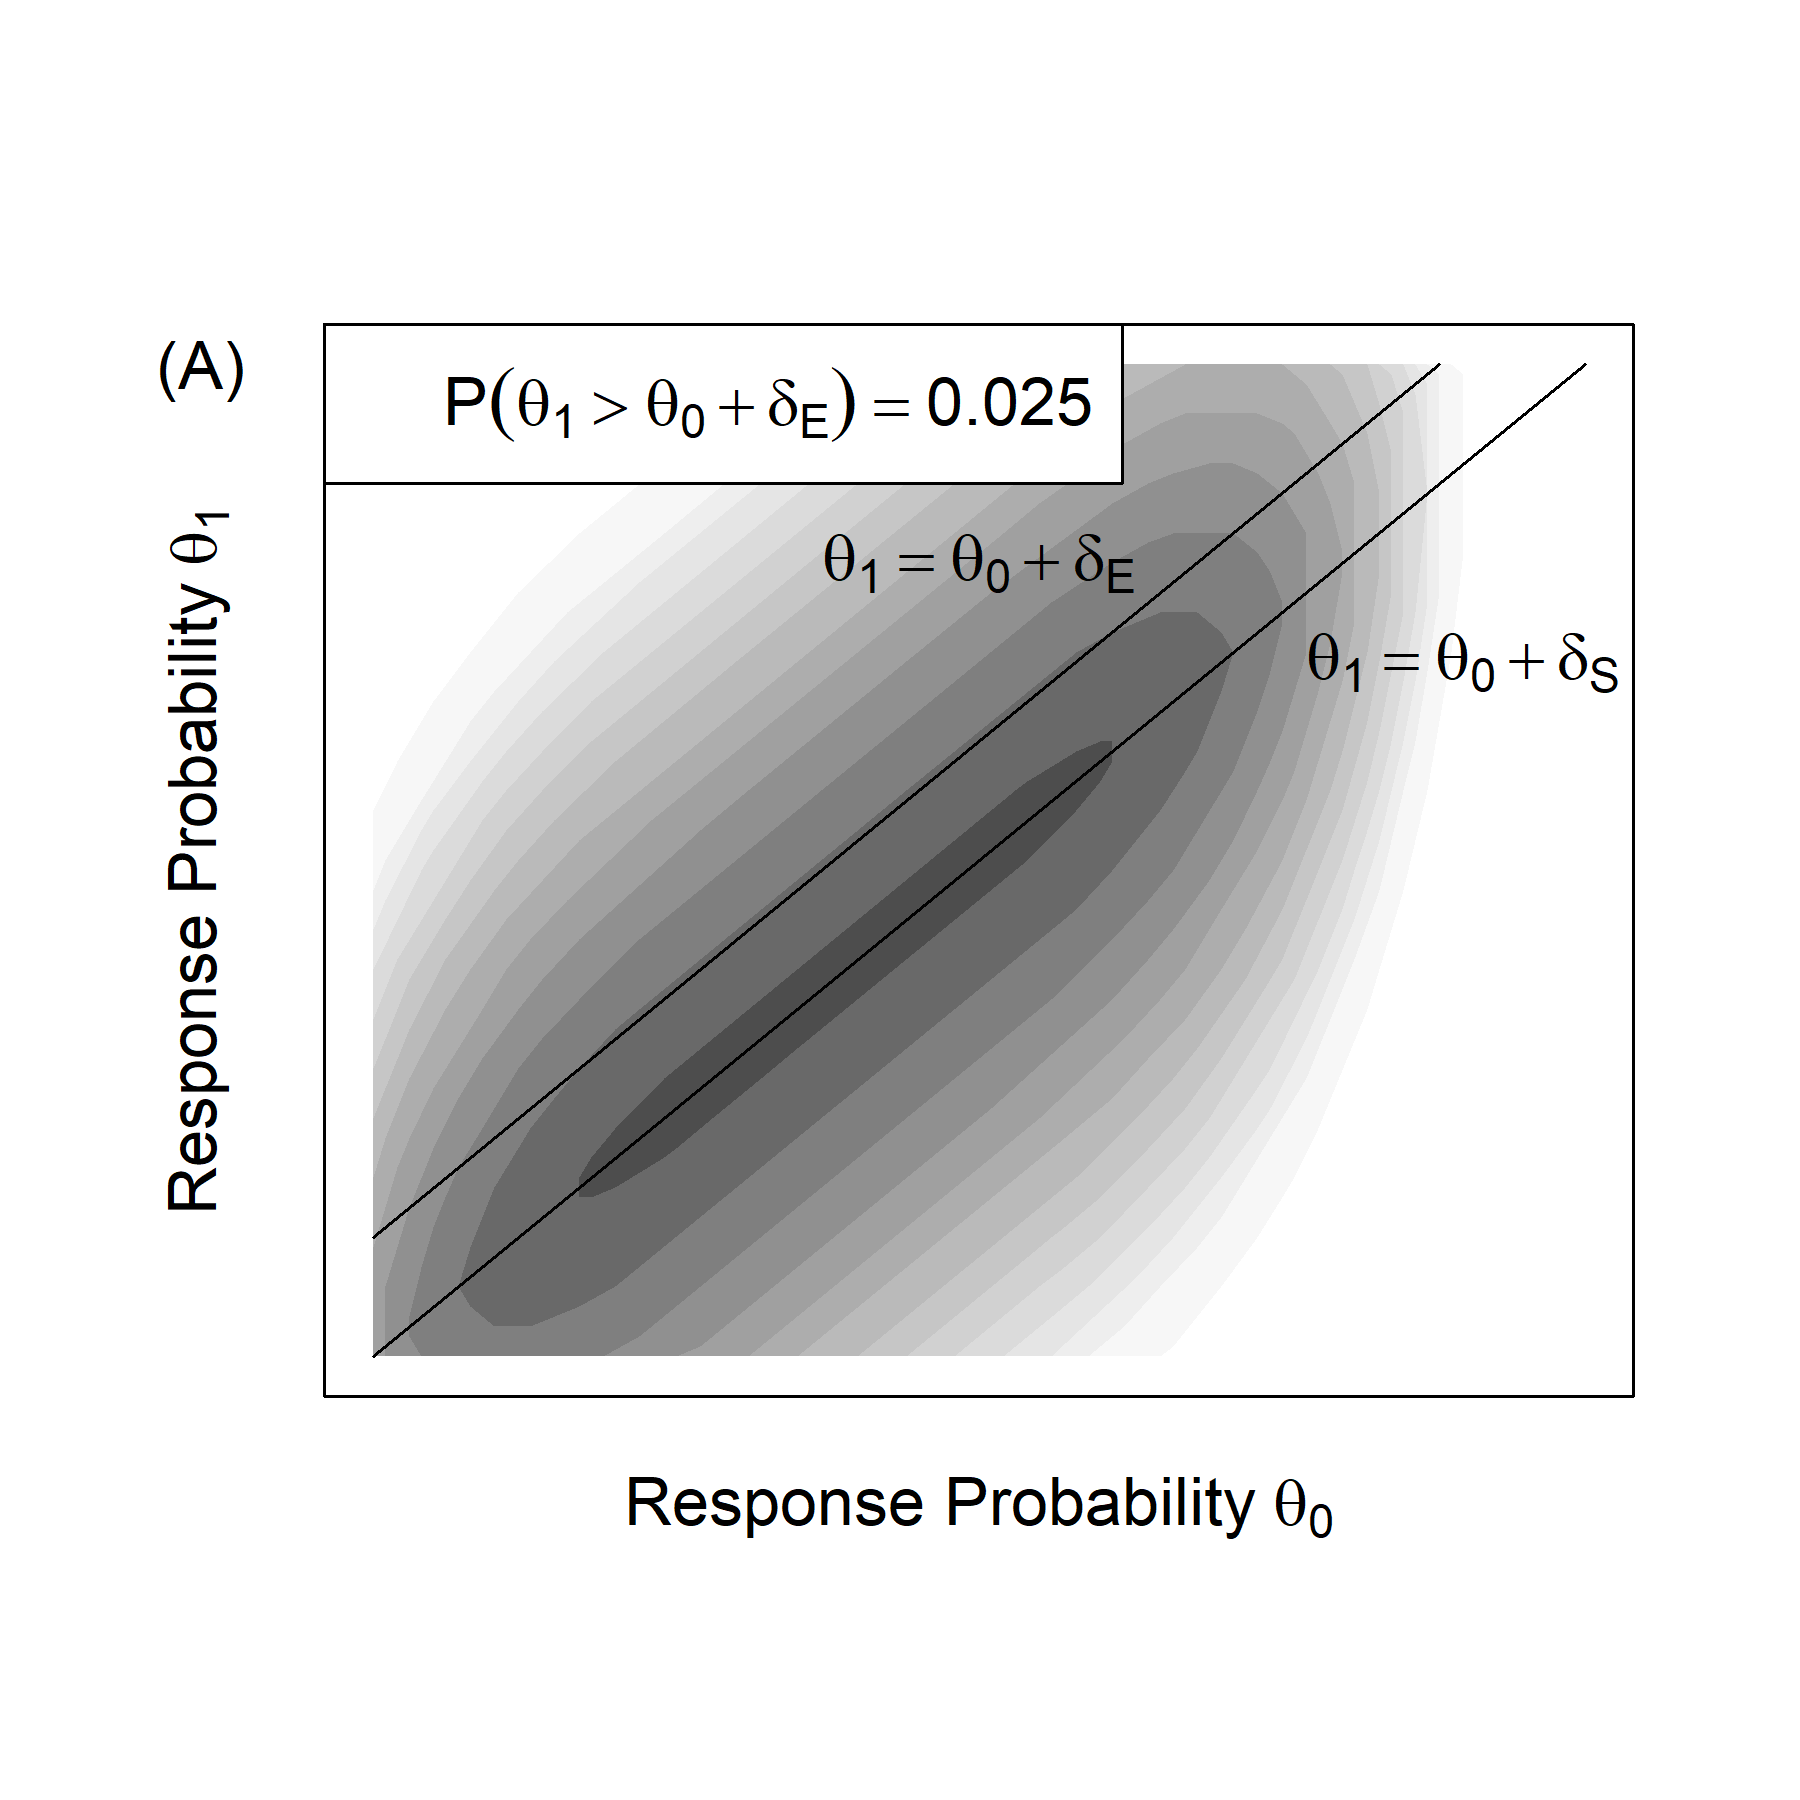
\includegraphics[width=6in]{../00-paper/FIGURES/figure5a.png}
%%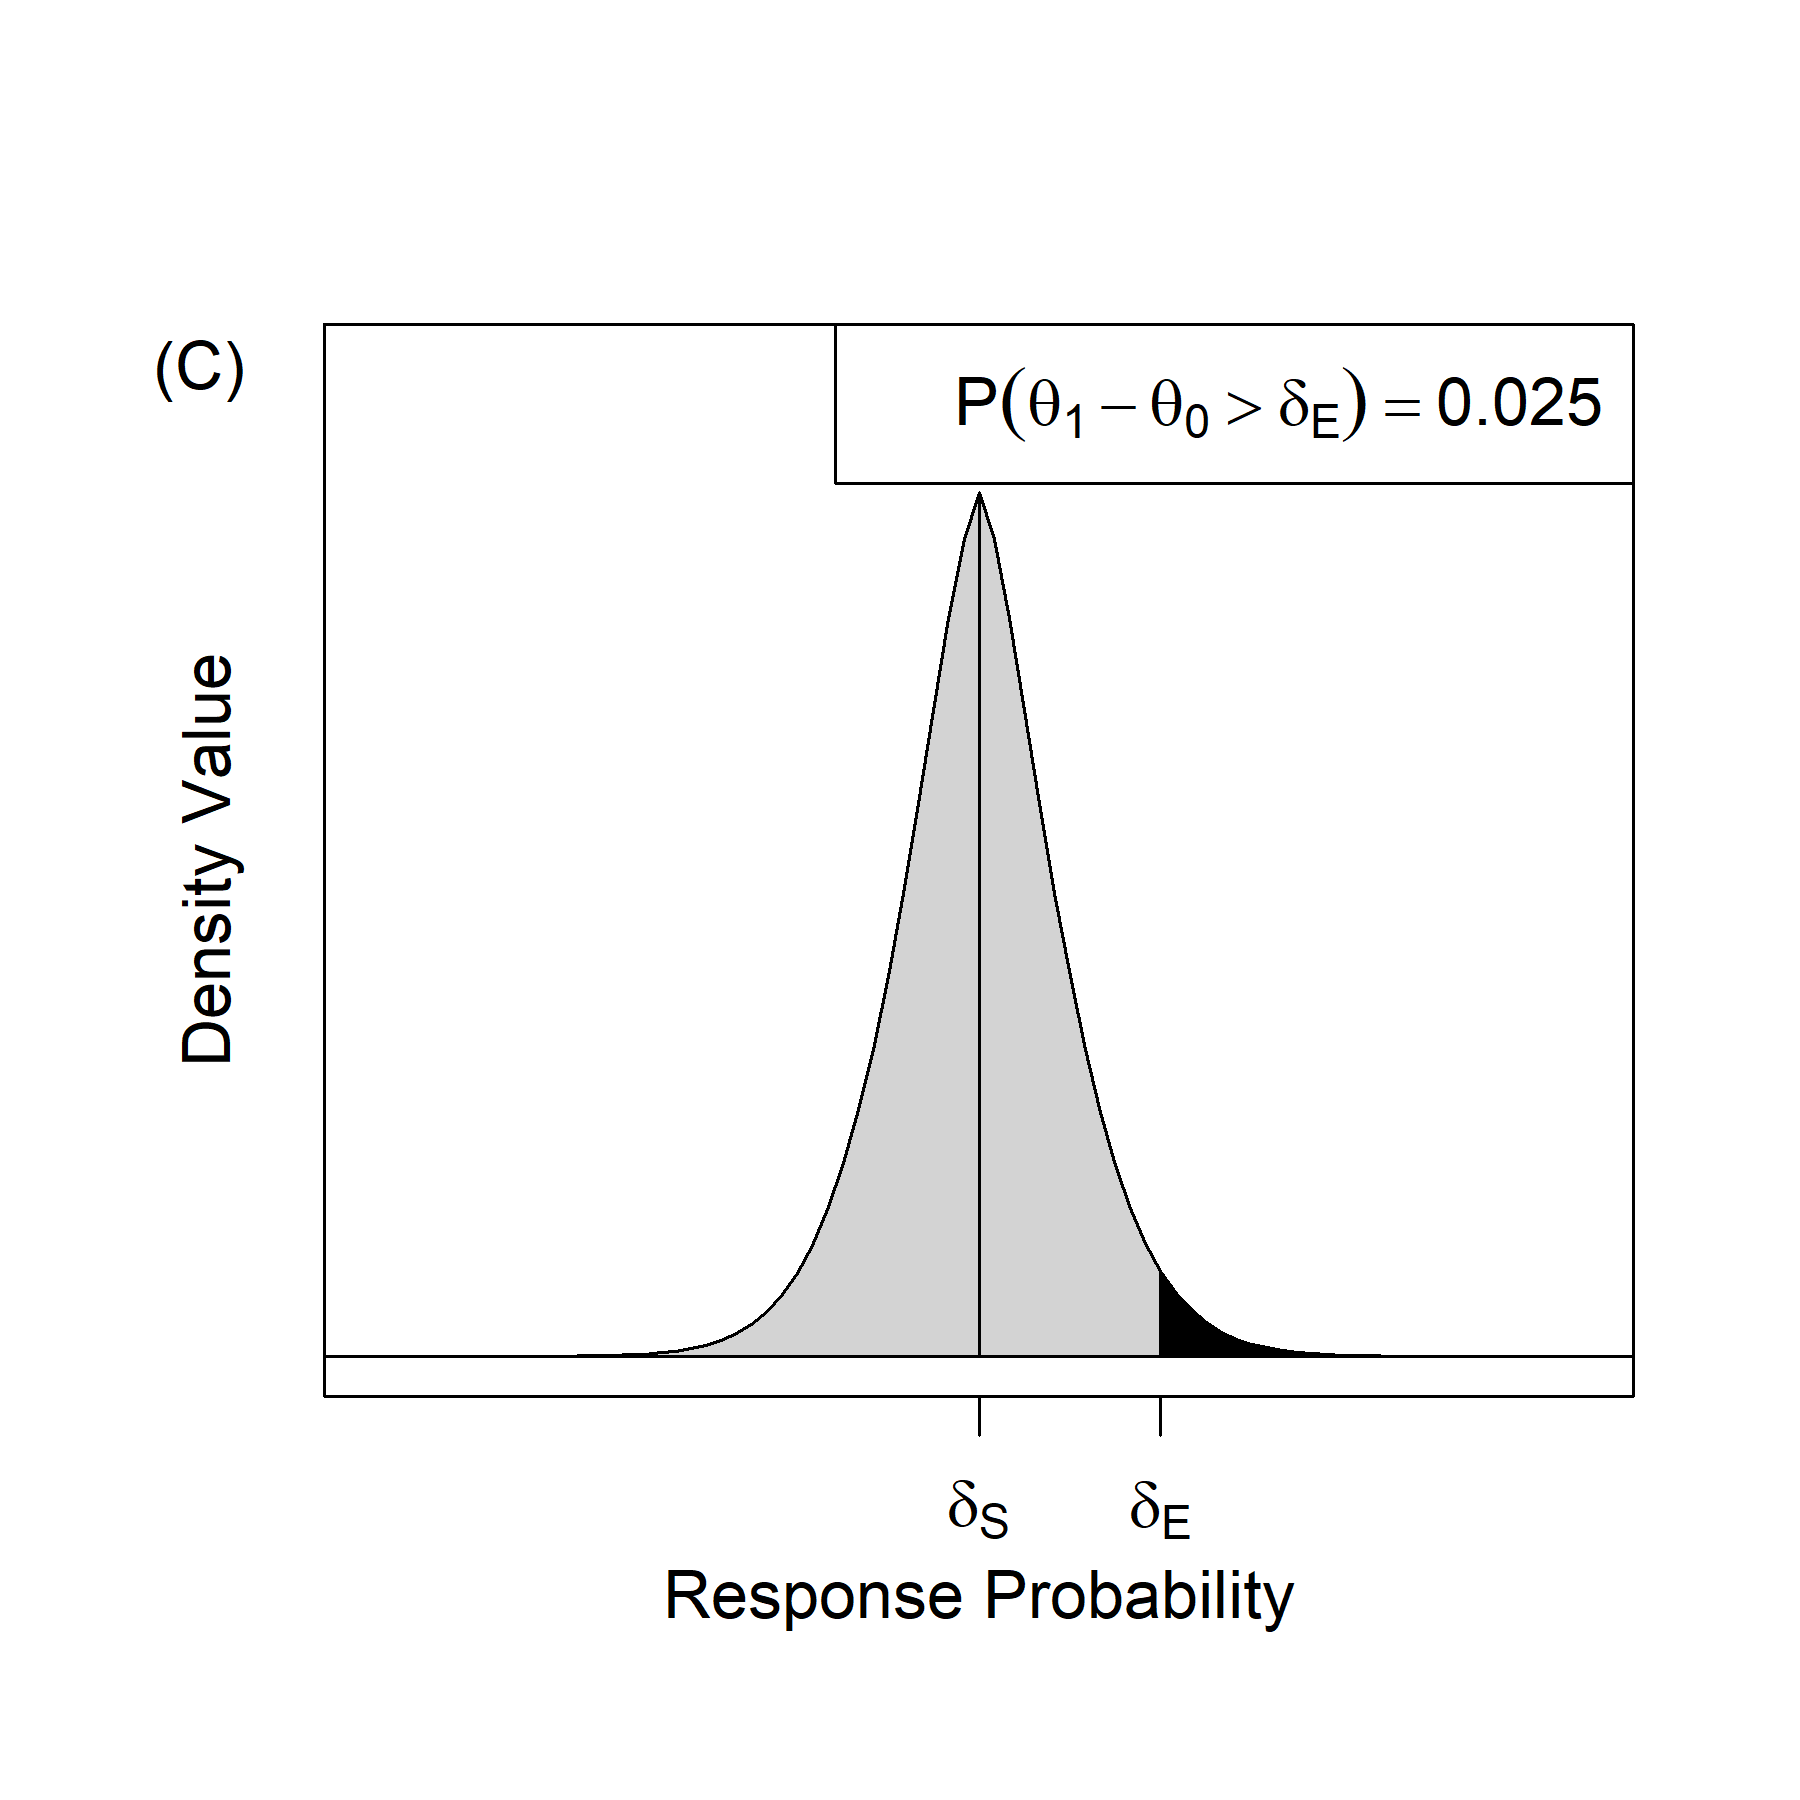
\includegraphics[width=3in]{../00-paper/FIGURES/figure5d.png}
%%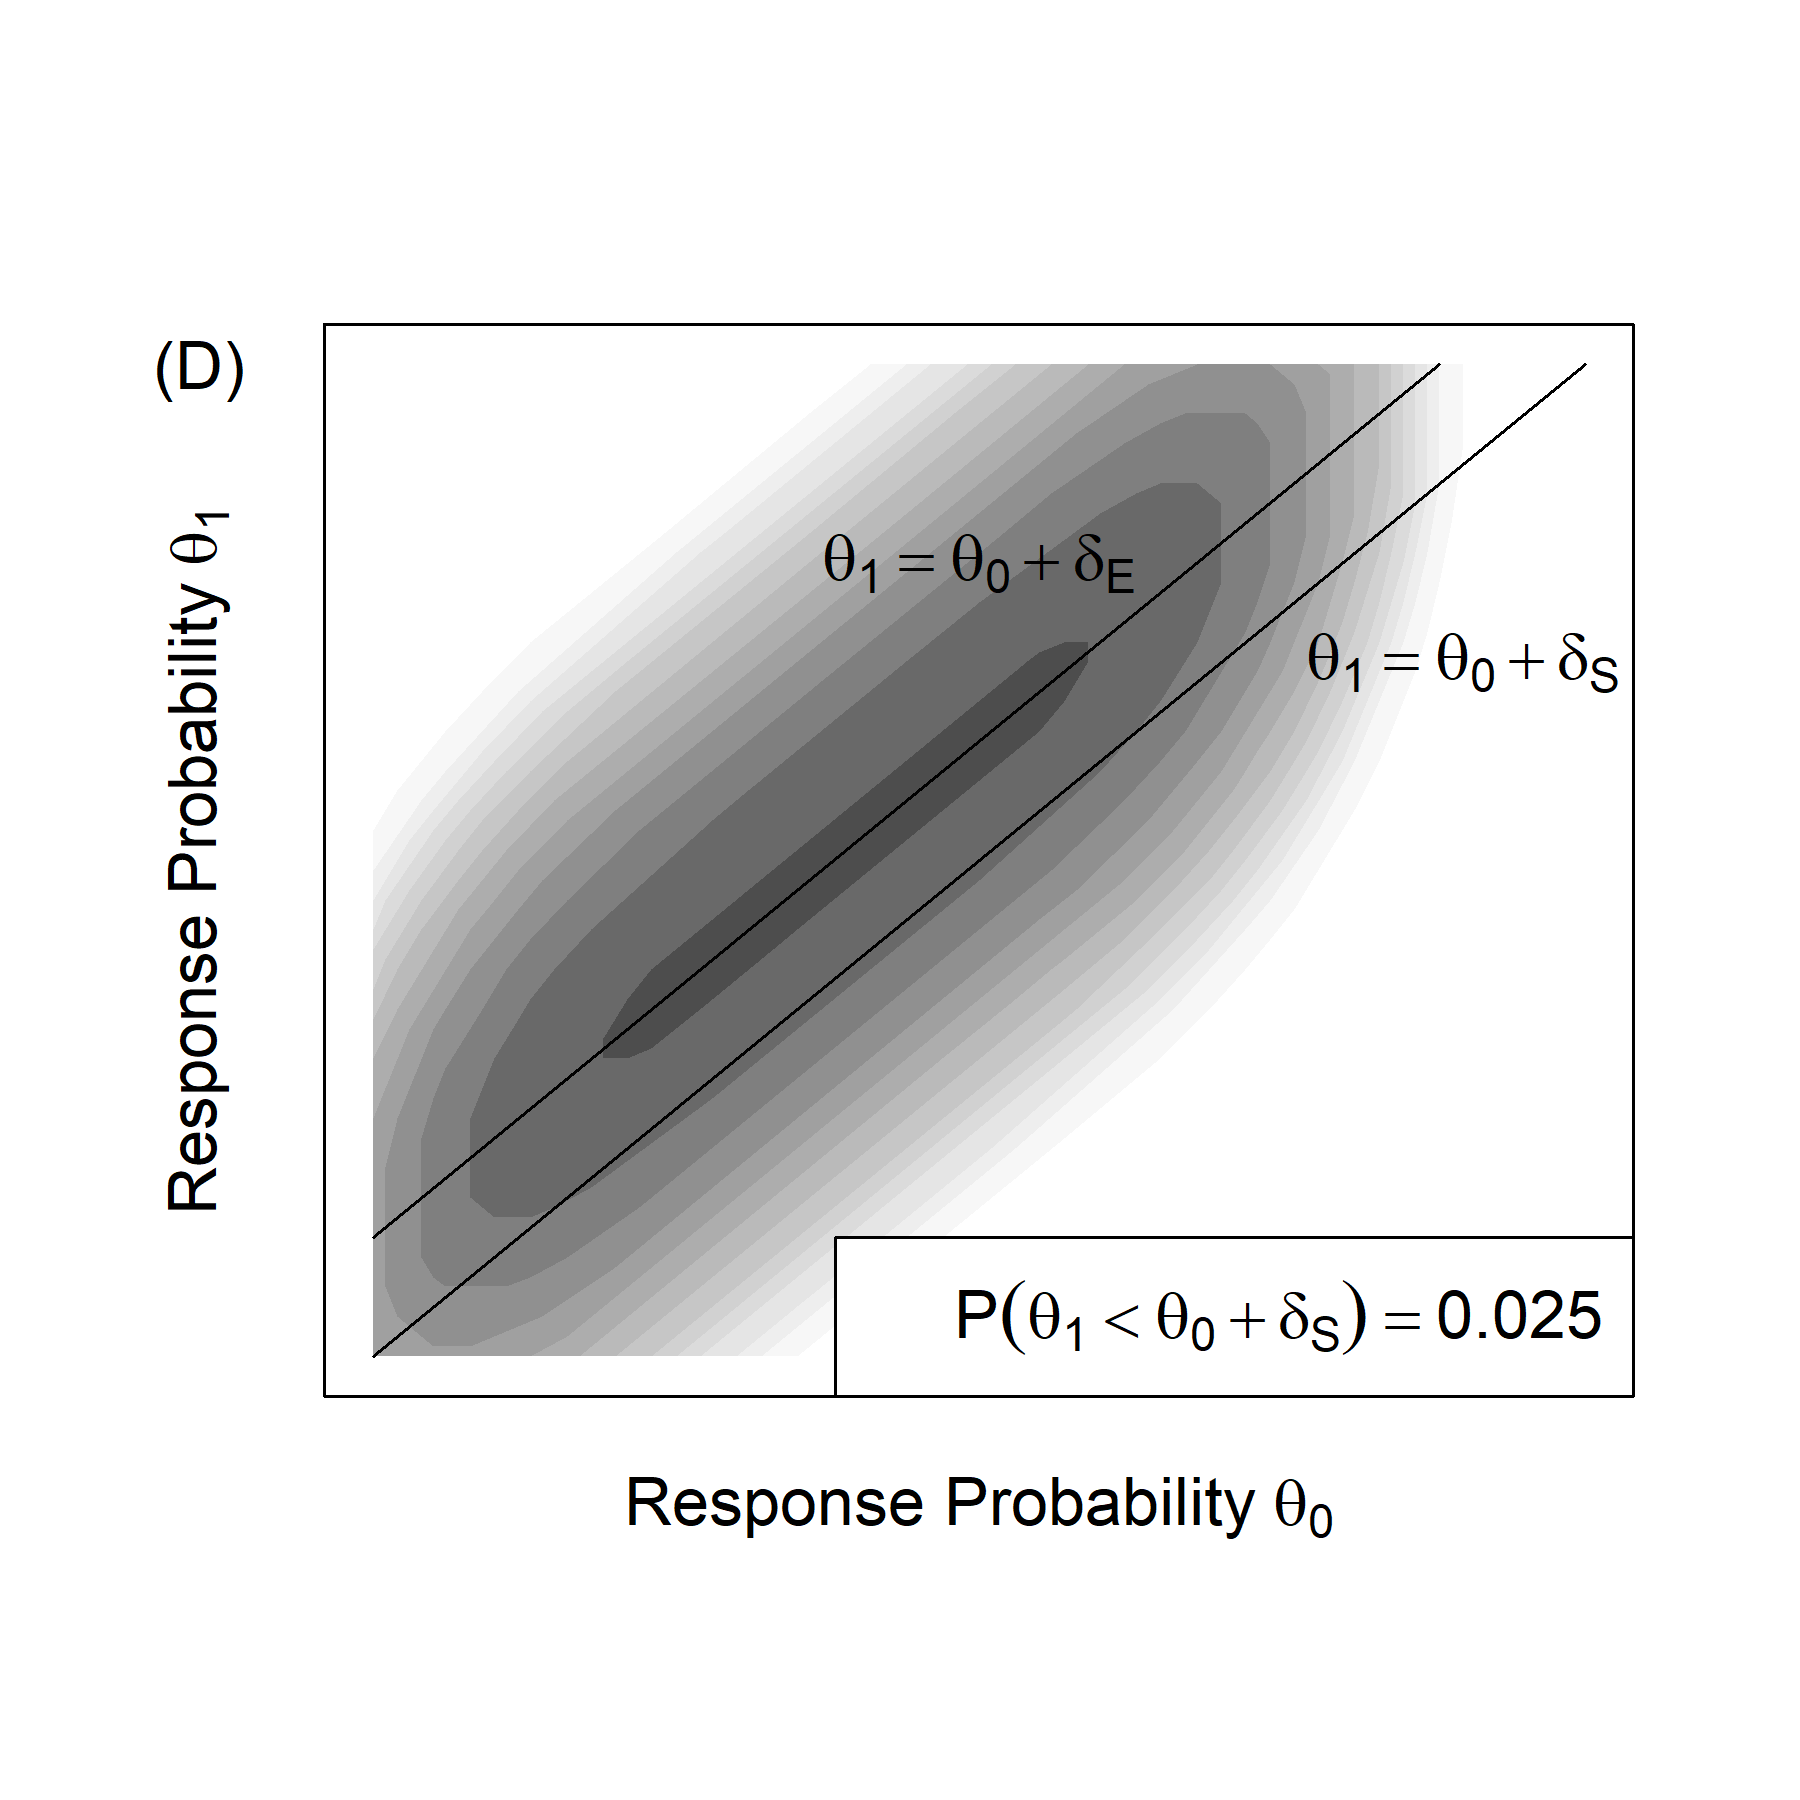
\includegraphics[width=3in]{../00-paper/FIGURES/figure5b.png}
%%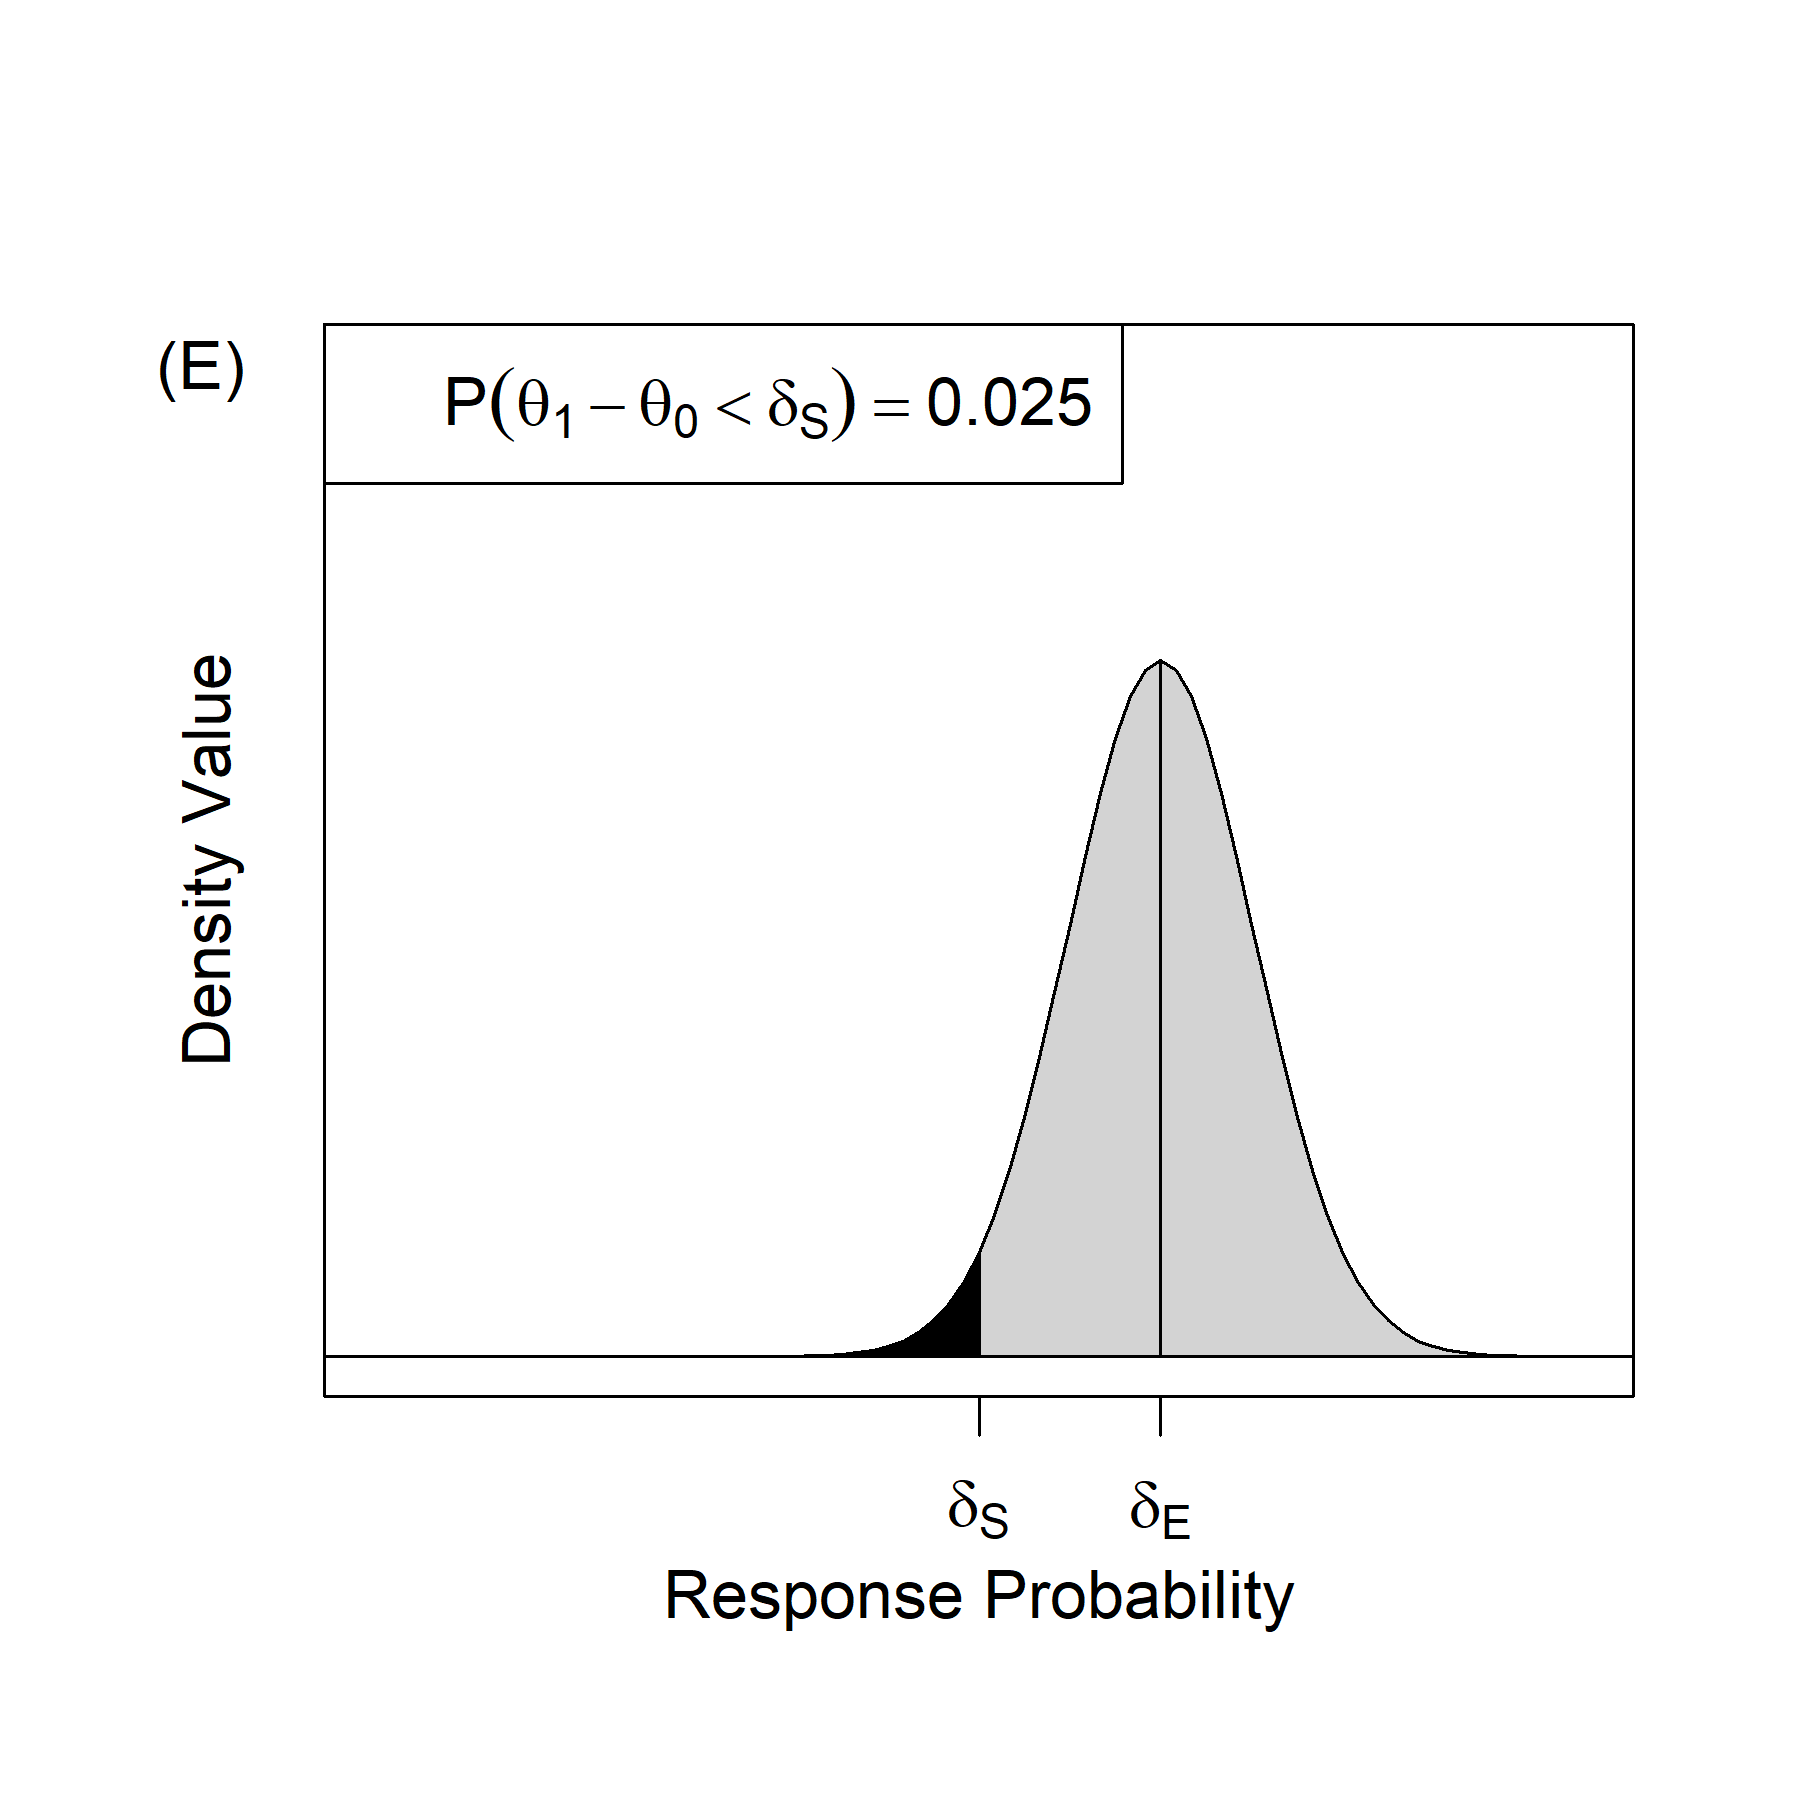
\includegraphics[width=3in]{../00-paper/FIGURES/figure5e.png}
%\caption{Joint distribution $\pi(\theta,\eta)=\pi(\theta)\times\pi(\eta|\theta)$, where $
%\pi(\theta)\sim\mathcal{GN}_{p=0.975,\Theta=[-1,1]}(\tilde{\mu}=\theta_0,q=\theta_1,\gamma=1)$ and $\pi(\eta|\theta)\sim \mathcal{GN}_{p=0.975,H=[\rmn{max}(-\theta,0),\rmn{min}(1,1+\theta)]}(\tilde{\mu}=\eta_0,q=\eta_1,\gamma=1)$.}
%\label{fig:figure5}
% \end{center}
%\end{figure}
%
%
%\subsection{Generalized Normal Cumulative Distribution Function}
%The CDF of a generalized normal random variable $\theta\sim\mathcal{GN}(\mu,\alpha,\beta)$ can be expressed as \citep{Griffin2018}
%\begin{equation}
%P(\theta\leq q|\mu,\alpha,\beta)=\frac{1}{2}+\frac{\rmn{sign}(q-\mu)}{2}\int_0^{|q-\mu|^\beta}\frac{w^{1/\beta-1}}{\alpha\Gamma(1/\beta)}\rmn{exp}\left\{-\left(\frac{1}{\alpha}\right)^\beta w\right\} dw
%\end{equation}
%\subsection{Parameterizing the $\mathcal{GN}_p(\tilde{\mu},q,\gamma)$ Distribution}
%The restrictions on the choice of $(p,\tilde{\mu},q,\gamma)$ for the $\theta\sim\mathcal{GN}_p(\tilde{\mu},q,\gamma)$ distribution to be well-defined:

\label{lastpage}

\bibliographystyle{biom} 
\bibliography{mybibilo}

\end{document}
